\section{任务四}
\subsection{5轮密钥恢复攻击}
根据第1)问得到的4轮高概率差分路线：
$$
\text{0x}0001\longrightarrow\text{0x}0010
$$
阐述5轮密钥恢复攻击的基本过程：这里采用4+1轮模式，即在4轮高概率差分的末尾添加一轮。其中选择的明文对$(P,P')$满足
$$
P \oplus P' = \Delta_{in} = \text{0x}0001
$$
由高概率差分可知，四轮加密后相应输出$(C_4,C_4')$满足
$$
C_4 \oplus C_4' = \Delta_{out} = \text{0x}0010
$$
概率为0.049，远大于随机情况的$1/2^{16}$。探测其中第四轮加密结果这一中间情况的方法就是猜测第五轮的轮密钥$k_5$：
\begin{itemize}
    \item 若猜对$k_5$，则由五轮加密的到的密文$(C,C')$解密回正确的$(C_4,C_4')$，满足$C_4 \oplus C_4' = \text{0x}0010$的概率为高概率的0.049；
    \item 若猜错，则计算出来的$(C_4,C_4')$是错误的/随机的，以随机概率满足，即$\text{Pr}(C_4 \oplus C_4' = \text{0x}0010) = \frac{1}{2^{16}}$。
\end{itemize}
因此基本密钥恢复方法为随机选择$m$对满足输入差分的明文对，对$k_5$的每一种可能设置一个计数器，满足:
$$
S^{-1}(C\oplus k_5) \oplus S^{-1}(C'\oplus k_5) = \Delta_{out}
$$
的则令计数器值+1，处理完$m$对明文后，正确密钥的计数将明显高于错误密钥的计数，从而恢复出正确的密钥。

但是我们注意到，并非所有输入对$(P,P')$都能满足在四轮加密后满足$C_4 \oplus C_4' = \Delta_{out}$，这样不满足的对称为错误对，恢复密钥攻击实际要使用的是正确对，错误对会对密钥恢复造成干扰，有以下事实：
\begin{itemize}
    \item 正确对+正确密钥一定满足$C_4 \oplus C_4' = \Delta_{out}$；
    \item 正确对+错误密钥以随机概率满足$C_4 \oplus C_4' = \Delta_{out}$；
    \item 错误对+正确密钥一定不满足上式，即$C_4 \oplus C_4 ' \not = \Delta_{out}$；
    \item 错误对+错误密钥以随机概率满足$ C_4 \oplus C_4' = \Delta_{out}$。
\end{itemize}
因此结合采样、去噪、恢复密钥三个步骤来筛选正确对，提高密钥恢复的成功概率。
\begin{itemize}
    \item 采样：随机选择明文$P$，计算$P' = P \oplus (\text{0x}0001)$，重复该过程$m$次，得到$m$对满足输入差分的明文对，做5轮CipherFour算法加密得到对应的密文对。我们期望得到/留下的是正确对，满足$C_4 \oplus C_4' = \text{0x}0010$，其中发现过$S$盒子的输入0差分，输出还是0差分；且查过S盒的DDT后发现
输入差分为1时，输出差分只可能是$1,2,5$,因此5轮加密后正确对应满足:
$$
\begin{cases}
    \Delta C_{5,0} = \Delta C_{5,1} = \Delta C_{5,3} = 0\\
    \Delta C_{5,2} = \text{0x}1/\text{0x}2/\text{0x}5
\end{cases}
$$
    \item 去噪：按照上面的分析，对$m$对密文，计算器差分值$\Delta C_5$，保留满足:
    $$
    \Delta C_5 \in \{  \text{0x}0,\text{0x}0  ,h,\text{0x}0 | h \in \{\text{0x}1,\text{0x}2,\text{0x}5\} \}
    $$
    注意这里保留的逻辑是，正确对一定满足上式所以被保留，特殊错误对(比如四轮加密中间值其他(第1，2，4)字节差分为0、第3半字差分并非为$\text{0x}1$的错误对也满足过$S$盒后为$h$)能满足上式而被保留，大部分错误对被排除掉，因此去噪后并不是所有留下的都是正确对，但能显著提高正确对的占比。
    \item 恢复密钥：设去噪后有$\epsilon n$对密文保留下来，记最后一轮第三个$S$盒相应的密钥为$k_{5,2}$，我们的目标就是恢复这一4bit密钥（实际上由于其他3个S盒的输入差分都为0差分，因此任何密钥都能满足输入零差分到输出零差分，缺少有效信息恢复密钥其他比特），对每一对密文信息建立共$\epsilon n$个下述方程:
    $$
    S^{-1}(C_{5,2}) \oplus S^{-1} (C'_{5,2} \oplus k_{5,2}) = \text{0x}1
    $$
    按照前面的密钥计数器方法，保留前$2^{4-a}$个作为正确密钥的候选值。对于上述方程的求解，不妨转成正向方程来看:
    $$
    S(x \oplus k ) \oplus S(x' \oplus k) = \beta
    $$
    其中$S$为过S盒查表运算，$(x,x',\beta)$已知(在这里$(x,x')$就是四轮加密中间值，$\beta$就是五轮加密后最终密文对的差分)。一种方法是穷举$k$的所有可能，代入方程进行验证；另一种方法为借助$S$盒的差分分布表求解：
    记$ \oplus x' = \alpha$，$S$盒的所有满足输入差分为$\alpha$、输出差分为$\beta$的可能输入集合为$IN_S(\alpha,\beta)$，得到的候选密钥集合为
    $\{ x \oplus X | X \in IN_S(\alpha,\beta)  \}$

\end{itemize}

\subsubsection{代码运行结果}

首先运行明密文文件验证程序。使用实验指导书给出的六个密钥字
$$
(\text{0x}0123,\text{0x}4567,\text{0x}89AB,\text{0x}CDEF,\text{0x}FEDC,\text{0x}BA98)
$$

这里先用上述六个轮密钥重新加密文件中的 $2^{16}$ 个明文，计算发现密文与文件中的密文全部匹配。随后将最后一个密钥字的最后一个半字节由 $\text{0x}8$ 改为 $\text{0x}9$，得到 $K_6=\text{0x}BA99$，此时 $2^{16}$ 个密文全部不匹配。这个对照确认了本地文件确实对应指导书给出的密钥组和当前采用的加密结构，为后续筛选及密钥枚举提供了匹配的实验数据。
\begin{figure}[H]
    \centering
    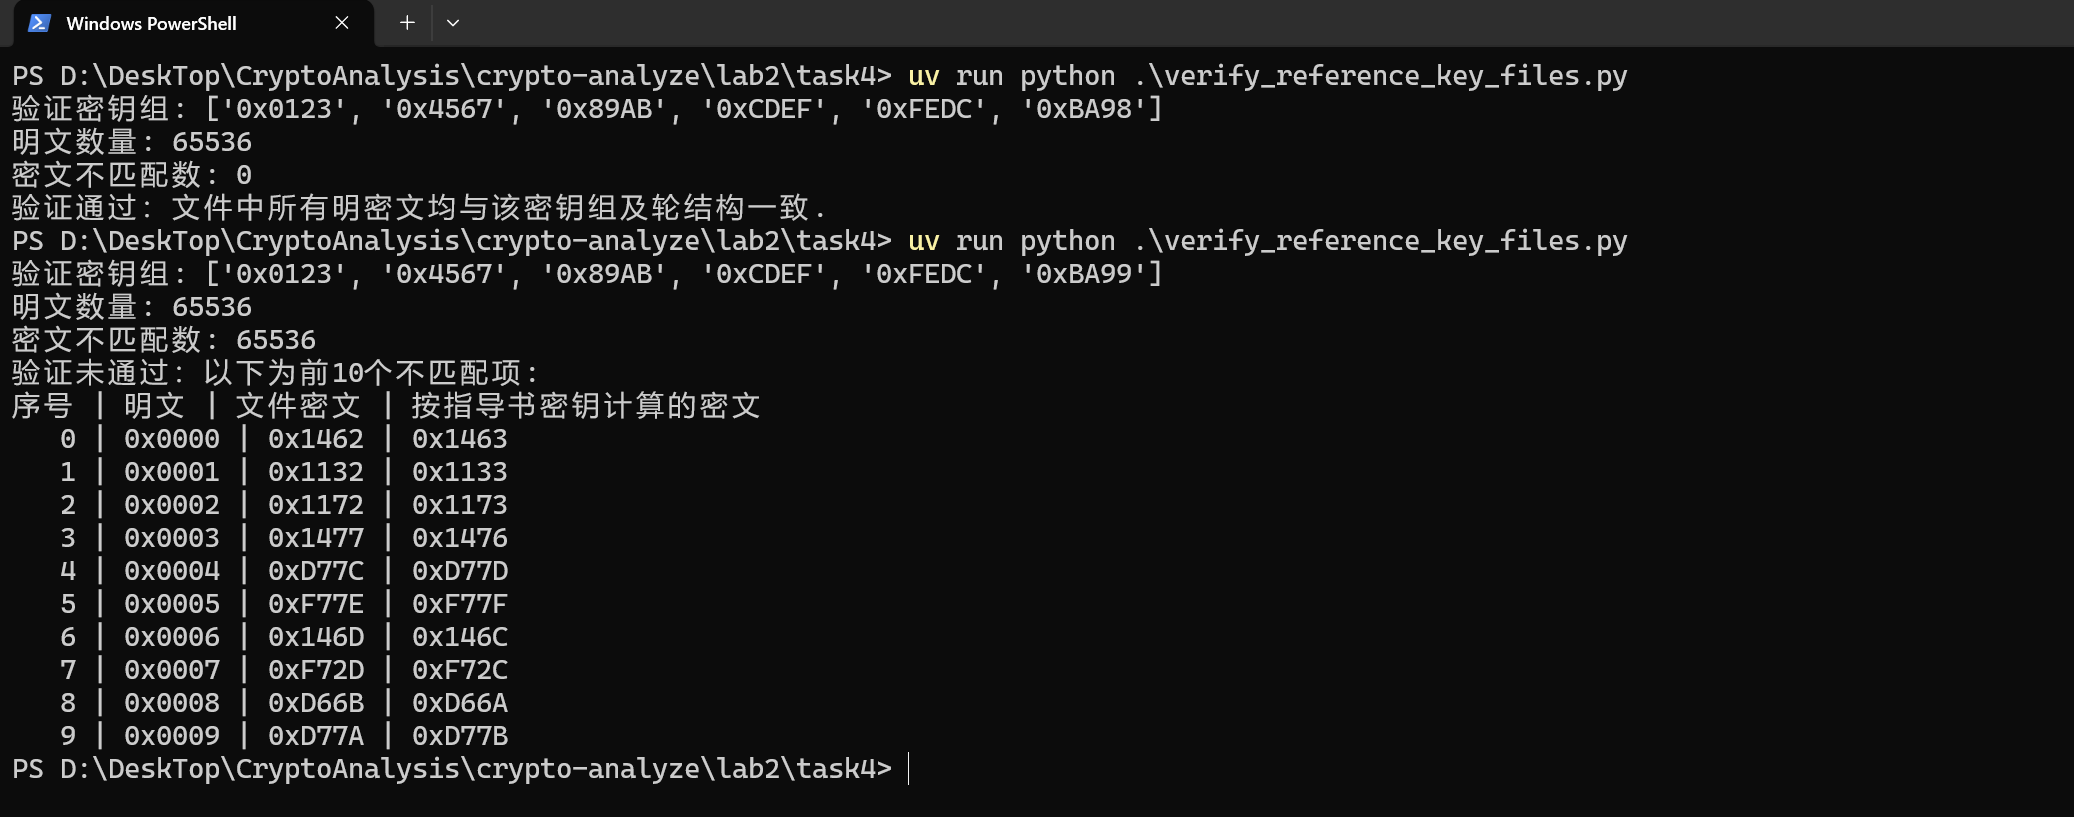
\includegraphics[width=0.96\textwidth]{figures/task4_verify_key.png}
    \caption{验证指导书密钥与明密文文件的对应关系}
\end{figure}

在已验证的明密文文件上运行密文筛选和半字节密钥枚举程序。筛选后保留 $4028$ 对，去噪前正确对占比约$4.8\%$，去噪后占比
$$
\frac{2^{16} \times 0.048}{4028} \approx 78\%
$$
正确对占比显著提高。
程序对目标半字节的 $2^4 = 16$ 种取值逐一计数。根据给定密钥 $K_6=\text{0x}BA98$，目标半字节为 $\text{0x}9$。它的计数达到最高值 $3172$，与错误候选 $\text{0x}8$ 并列。因此，本次枚举将正确的 4 bit 半字节包含在最高分候选中；当前计数结果还不能在 $\text{0x}8$ 和 $\text{0x}9$ 之间作出唯一判断。候选计数如下：
\begin{table}[H]
    \centering
    \small
    \caption{恢复目标半字节的候选计数}
    \begin{tabular}{c r}
        \hline
        半字节候选 & 计数 \\
        \hline
        $\text{0x}8,\text{0x}9$ & 3172 \\
        $\text{0x}C,\text{0x}D$ & 1902 \\
        $\text{0x}0,\text{0x}1$ & 1544 \\
        $\text{0x}A,\text{0x}B$ & 1468 \\
        $\text{0x}2,\text{0x}3$ & 1268 \\
        $\text{0x}4,\text{0x}5$ & 1232 \\
        $\text{0x}6,\text{0x}7$ & 956 \\
        $\text{0x}E,\text{0x}F$ & 198 \\
        \hline
    \end{tabular}
\end{table}
\begin{figure}[H]
    \centering
    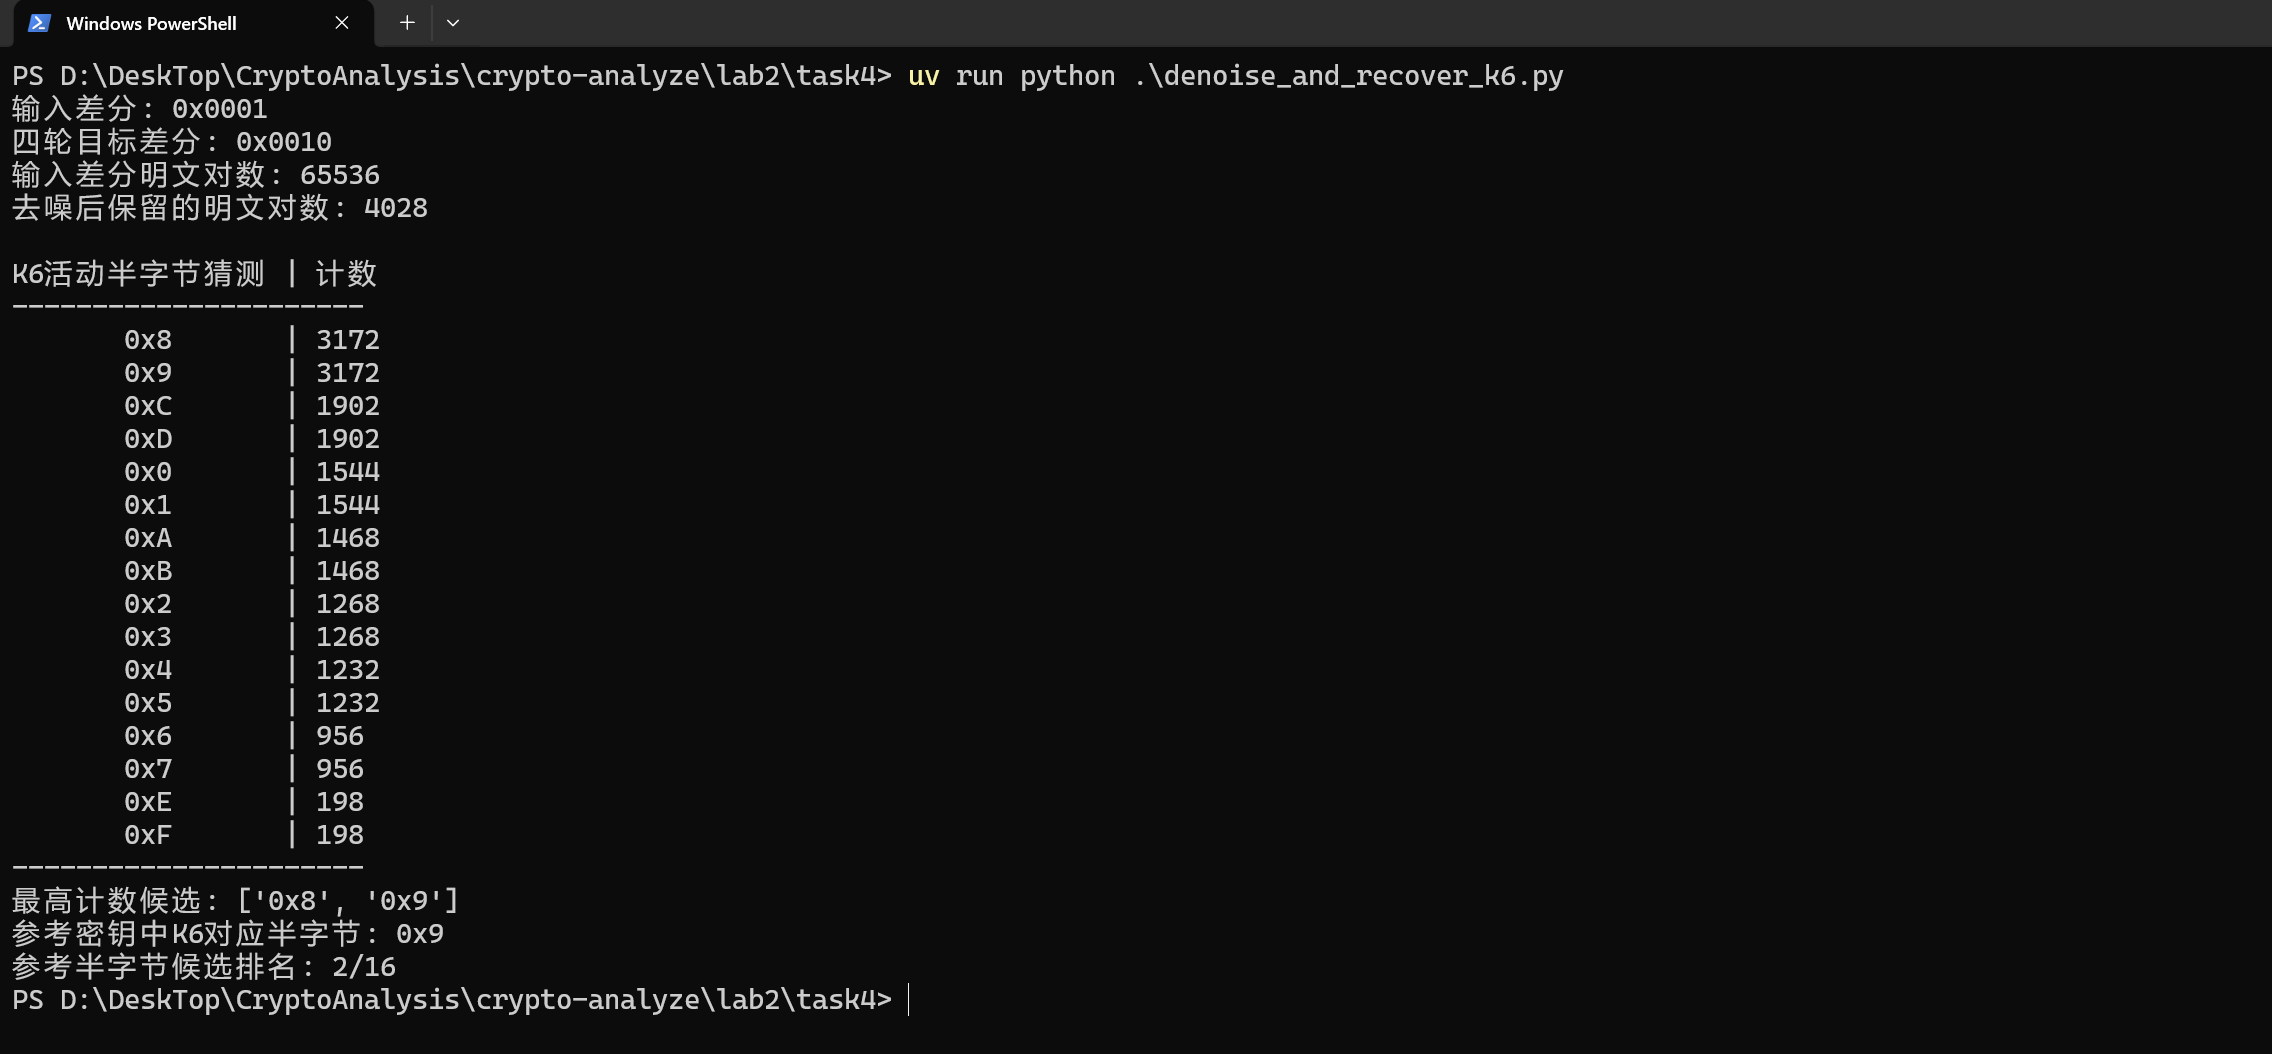
\includegraphics[width=0.96\textwidth]{figures/task4_find_sicret_key.png}
    \caption{筛选后对目标半字节进行差分计数的结果}
\end{figure}

随后对五组新生成的六字密钥重复筛选实验。程序复用文件中的全部明文，但为每组六字密钥分别重新计算对应的五轮密文。任务一得到的四轮差分理论概率为$p=0.0479736328125$；当$m=2^{16}$时，理论正确对数为
$$
mp=2^{16}\times0.0479736328125=3144.
$$
设某组密钥下实际筛选保留$N_j$对，则用$mp/N_j$估计保留对中正确对所占比例。五组统计结果如下：
\begin{table}[H]
    \centering
    \scriptsize
    \caption{五组新密钥下的筛选保留数及正确对占比估计}
    \begin{tabular}{c p{0.52\textwidth} r r}
        \hline
        组别 & 六字密钥组$(K_1,\ldots,K_6)$ & 实际保留数$N_j$ & $mp/N_j$ \\
        \hline
        1 & \texttt{[0x0E6B, 0x0286, 0xAD7C, 0x496C, 0xFEDE, 0x93AE]} & 3906 & 80.49\% \\
        2 & \texttt{[0x36B5, 0xC640, 0x98AB, 0x1A0C, 0x095F, 0xF3C0]} & 3702 & 84.93\% \\
        3 & \texttt{[0xC0E4, 0x3F92, 0x4112, 0x1D08, 0x734C, 0xFB64]} & 3836 & 81.96\% \\
        4 & \texttt{[0x49A0, 0x7650, 0x9B9A, 0xAE68, 0xAA6B, 0x1255]} & 3696 & 85.06\% \\
        5 & \texttt{[0x8108, 0x5E1F, 0x13DD, 0xA3D8, 0xE75D, 0xB84D]} & 3656 & 86.00\% \\
        \hline
    \end{tabular}
\end{table}
五组实际保留数的平均值为$3759.20$对，通过去噪阶段后正确对的平均占比为
$$
\frac{2^{16} \times 0.048}{3759.20} \approx 84\%
$$

\begin{figure}[H]
    \centering
    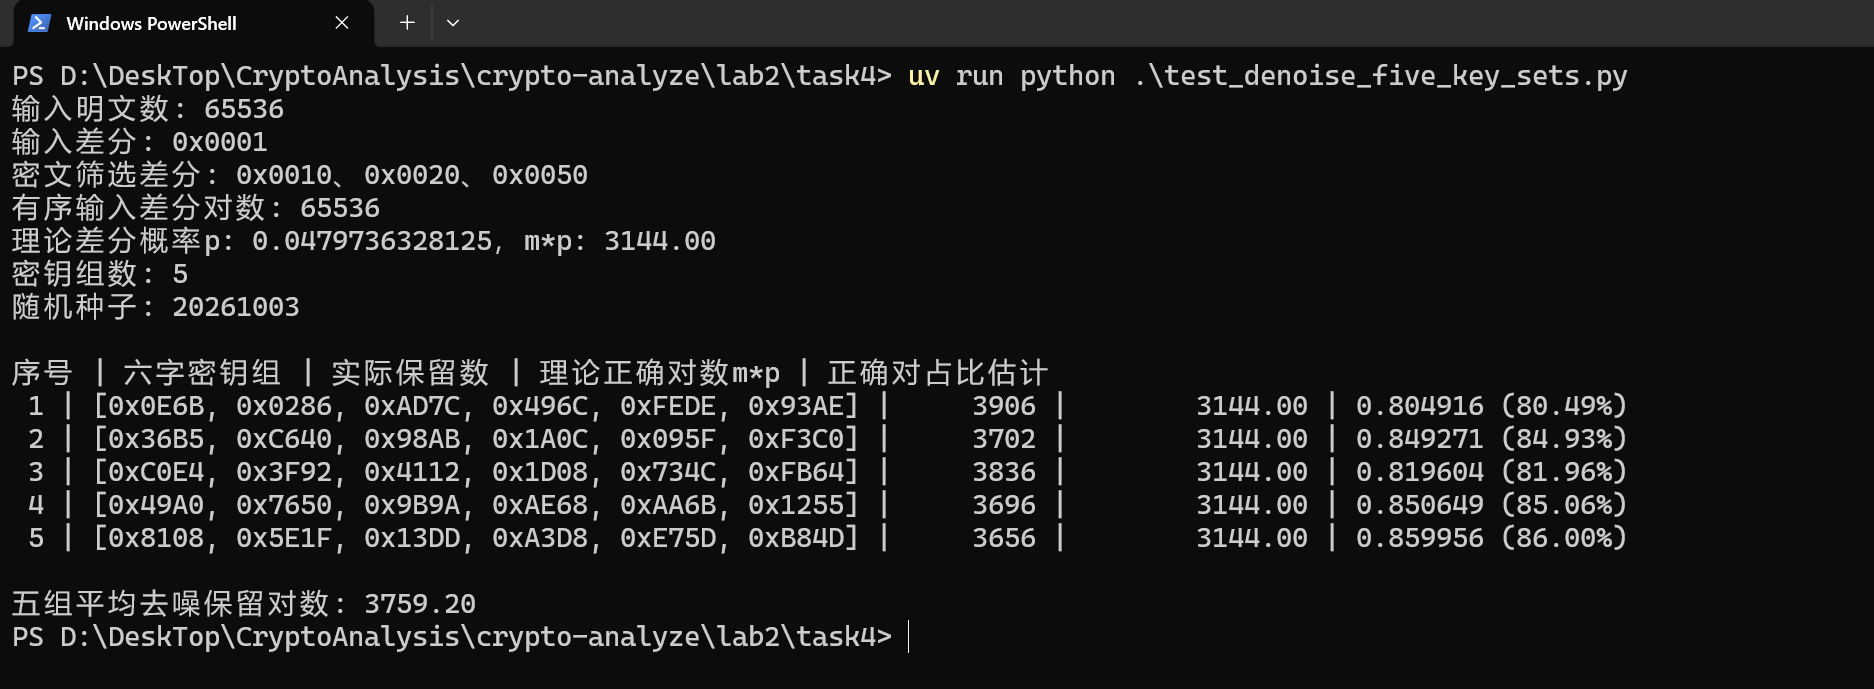
\includegraphics[width=0.96\textwidth]{figures/task4_other_key_sift_correct_pair.png}
    \caption{五组新密钥下的去噪保留数及正确对占比估计}
\end{figure}

\subsubsection{复杂度分析}
\begin{itemize}
    \item 数据复杂度：选择了$2^{16}$个明文对，即$2^{17}$个明文。
    \item 时间复杂度：
    \begin{itemize}
        \item 采样阶段要获得$2^{17}$个明文对应的密文，即做$2^{17}$次5轮CipherFour算法的加密运算；
        \item 去噪阶段计算$2^{16}$个密文对的差分值，即$2^{16}$次异或运算；
        \item 恢复密钥阶段：去噪后保留$\epsilon n$对密文，每个4 bit半字节有$2^4$种猜测。对每一种猜测，都需要逐一检查全部保留对，因此需要$2^4\times\epsilon n$次差分方程验证。本次保留$4028$对，对应$16\times4028=64448$次验证。
    \end{itemize}
    \item 存储复杂度：
    \begin{itemize}
        \item 采样阶段存储选择明文对应的密文，即$2^{17} \times 16 = 2^21\text{bit} = 256\text{KB}$；
        \item 4bit每种设置计数器，若每个计数器占8bit，则计数器的存储复杂度约为$2^4 \times 8 = 2^7\text{bit}$。
    \end{itemize}
\end{itemize}
% 筛选阶段对$m=2^{16}$个有序明文对逐一计算密文差分，时间复杂度为$O(m)$。设筛选后保留$N$对，对16种目标半字节猜测分别计数，时间复杂度为$O(16N)$；本次$N=4028$，需要约$16\times4028=64448$次半字节差分检查。程序保存明文到密文的对应关系及密文对，空间复杂度为$O(2^{16})$。
